% TODO: make it uniform the notation for sets (polyhedral set P clashes with problem P)

\section{Optimality for integer programming problems}

We will now discuss a method to solve mixed-integer programming problems that relies on the successive solution of linear programming relaxations. Although there are several methods that can be employed to solve combinatorial optimisation problems, most of them are not capable of providing optimality guarantees for the solution obtained (e.g., are heuristics or metaheuristics) or do not exploit the availability of a (linear) mathematical programming formulation. To date, the most widespread method that is capable of both is something that is generally known as a \emph{branch-and-cut} method.

Branch-and-cut methods are composed of a combination of multiple parts, including, among other techniques, a branch-and-bound approach, cutting planes, and heuristics as well. In the next chapters we will focus on each of these parts individually, starting with the branch-and-bound method.


\section{Relaxations}

Before we present the method itself, let us discuss the more general concept of \emph{relaxation}. We have visited the concept somewhat informally before, but now we will concentrate on a more concrete definition.

Consider an integer programming problem of the form
%
\begin{equation*}
	z = \mini_x \braces{c^\top x : x \in X \subseteq \integers^n}.
\end{equation*}
%
To prove that a given solution $x^*$ is optimal, we must rely on the notion of \emph{bounding}. That is, we must provide a pair of upper and lower bounds that are as close (or tight) as possible. In the occasion that these bounds are the same, and thus match the value of $z = c^\top x^*$, we have available a certificate of optimality for $x^*$. This concept must be familiar to you. We already used a similar arguments in Chapter \ref{chapter_5}, when we introduced the notion of dual bounds.

Most methods that can prove optimality work by bounding an optimal solution. In this context, bounding means to construct an increasing sequence of lower bounds
%
\begin{equation*}
	\underline{z}_1 < \underline{z}_2 < \dots < \underline{z}_s \leq z	
\end{equation*}
%
and a decreasing sequence of upper bounds
%
\begin{equation*}
	\overline{z}_1 > \overline{z}_2 > \dots > \overline{z}_t \geq z
\end{equation*}
%
to obtain as tight as possible lower ($\underline{z} \leq z$) and upper ($\overline{z} \geq z$) bounds. Notice that the process can be arbitrarily stopped when $\overline{z}_t - \underline{z}_s \leq \epsilon$, where $s$ and $t$ are some positive integers and $\epsilon > 0$ is a predefined (suitably small) tolerance. The term $\epsilon$ represents an \emph{absolute optimality gap}, meaning that one can guarantee that the optimal value is at most greater than $\underline{z}$ by $\epsilon$ units and at most smaller than $\overline{z}$ by $\epsilon$ units. In other words, the optimal value must be either $\underline{z}$, $\overline{z}$, or a value in between.

This framework immediately poses the key challenge of deriving such bounds efficiently. It turns out that this is a challenge that goes beyond the context of mixed-integer programming problems. In fact, we have already seen this idea of bounding in Chapter \ref{chapter_7}, when we discussed decomposition methods, which also generate lower and upper bounds during their execution.

Regardless of the context, bounds are typically of two types: \emph{primal} bounds, which are bounds obtained by evaluating a \emph{feasible} solution (i..e, that satisfy primal feasibility conditions); and \emph{dual} bounds, which are typically attained when a primal feasibility is allowed to be violated so that a dual feasible solution is obtained. In the context of minimisation, primal bounds are upper bounds (to be minimised), while dual bounds are lower bounds (to be maximised). Clearly, in the case of maximisation, the reverse holds. 

Primal bounds can be obtained by means of a feasible solution. For example, one can heuristically assemble a solution that is feasible by construction. On the other hand, dual bounds are typically obtained by means of solving a \emph{relaxation} of the original problem. We are ready now to provide Definition \ref{p1c9:def:relaxation}, which formally states the notion of a relaxation.

\begin{definition}[Relaxation] \label{p1c9:def:relaxation}
	A problem 
	%
	\begin{equation*}
	  (RP): z_{RP} = \mini \braces{\overline{c}^\top x : x \in \overline{X} \subseteq \reals^n} 
	\end{equation*}
%
	is a \emph{relaxation} of problem
	%
	\begin{equation*}
	  (P): z = \mini \braces{c^\top x : x \in X \subseteq \reals^n} 
	\end{equation*}
	%
	if $X \subseteq \overline{X}$, and $\overline{c}^\top x \leq c^\top x$, $\forall x \in X$.
\end{definition}

Definition \ref{p1c9:def:relaxation} provides an interesting insight related to relaxations: they typically comprise an expansion of the feasible region, possibly combined with an objective function bounding. Thus, two main strategies to obtain relaxations are to enlarge the feasible set by dropping constraints and replacing the objective function with another of same or smaller value. One might notice at this point that we have used a very similar argumentation setting to define linear programming duals in Chapter \ref{chapter_5}. We will return to the relationship between relaxations and Lagrangian duality in a more general setting in Part \ref{part_2}, when we discuss the notion of Lagrangian relaxation.

Clearly, for relaxations to be useful in the context of solving mixed-integer programming problems, they have to be easier to solve than the original problem. That being the case, we can then rely on two important properties that relaxations have, which are crucial for using them as a means to generate dual bounds. These are summarised in Proposition \ref{p1c9:prop:relaxation_bounding} and \ref{p1c9:prop:relaxation_optimality}.

\begin{proposition} \label{p1c9:prop:relaxation_bounding}
	If RP is a relaxation of P, then $z_{RP}$ is a dual bound for $z$. 
\end{proposition}
    
\begin{proof} For any optimal solution $x^*$ of $P$, we have that $x^* \in X \subseteq \overline{X}$, which implies that $x^* \in \overline{X}$. Thus, we have that
  \begin{equation*}
  	 z = c^\top x^* \geq \overline{c}^\top x^* \geq z_{RP}.	\qedhere
  \end{equation*}
\end{proof}

The first inequality is due to Definition \ref{p1c9:def:relaxation} and the second is because $x^*$ is simply a feasible solution, but not necessarily the optimal, for $z_{RP}$. 

\begin{proposition} \label{p1c9:prop:relaxation_optimality}
  The following statements are true:
  \begin{enumerate}
  	\item If a relaxation RP is infeasible, then P is infeasible. 
  	\item Let $x^*$ be an optimal solution for RP. If $x^* \in X$ and $\overline{c}^\top x^* = c^\top x^*$, then $x^*$ is an optimal solution for P.
  \end{enumerate}
\end{proposition}
%
\begin{proof}
    To prove (1), simply notice that if $\overline{X} = \emptyset$, then $X = \emptyset$. To show (2), notice that as $x^* \in X$, $z \leq c^\top x^* = \overline{c}^\top x^* = z_{RP}$. From Proposition \ref{p1c9:prop:relaxation_bounding}, we have $z \geq z_{RP}$. Thus, $z = z_{RP}$. 
\end{proof}


\subsection{Linear programming relaxation}

In the context of solving (mixed-)integer programming problems, we will rely on the notion of linear programming (LP) relaxations. We have briefly discussed the idea in the previous chapter, but, for the sake of precision, let us first define what we man by the term. 

\begin{definition}[Linear programming (LP) relaxation]
  The LP relaxation of an integer programming problem $\mini \braces{c^\top x : x \in P \cap \integers^n}$ with $P = \braces{x \in \reals^n_+ : Ax \leq b}$ is the linear programming problem $\mini \braces{c^\top x : x \in P}$.
\end{definition} 

Notice that an LP relaxation is indeed a relaxation, since we are enlarging the feasible region by dropping the integrality requirements while maintaining the same objective function (cf. Definition \ref{p1c9:def:relaxation}).

Let us consider a numerical example. Consider the integer programming problem
% 
\begin{align*}
	z = \maxi_x ~& 4x_1 -x_2 \\
	\st &  7x_1 -2x_2 \leq 14 \\
	    & x_2 \leq 3 \\
	    & 2x_1 - 2x_2 \leq 3\\
	    & x \in \integers^2_+. 
\end{align*}

A dual (upper; notice the maximisation) bound for $z$ can be obtained by solving its LP relaxation, which yields the bound $z_{LP} = 8.42 \ge z$. A primal (lower) bound can be obtained by choosing any of the feasible solutions (e.g., $(2,1)$, to which $z = 7 \le z$). This is illustrated in Figure \ref{p1c9:fig:LP_relaxation}.

%TODO: Redraw figure in Julia.
\begin{figure}[h]
	\centering
	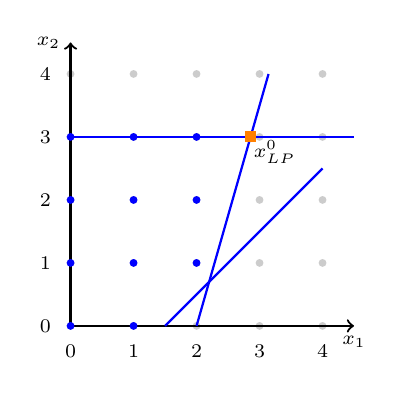
\begin{tikzpicture}[scale = 0.8,
	point/.style={circle, fill=gray!40, inner sep=1pt},
	feas point/.style={circle, fill=blue, inner sep=1pt}]
	%\draw[help lines] (0,0) grid (4,4);  
		\foreach \x in {0,...,4}{
		  \foreach \y in {0,...,4} {
		      \node[point] (\x,\y) at (\x, \y) {};
		  }}
		\foreach \x in {0,...,4}{
		  \node[font=\scriptsize] at (\x,-0.4) {$\x$};
		}
		\foreach \y in {0,...,4}{
		  \node[font=\scriptsize] at (-0.4,\y) {$\y$};
		}                      
		\draw[thick, <->] (4.5,0) node[below, font=\scriptsize]{$x_1$} -- (0,0) -- (0,4.5) node[left, font=\scriptsize]{$x_2$};    
		\draw[domain=0:4.5, thick, variable=\x, blue] plot ({\x},{3});
		\draw[domain=2:22/7, thick, variable=\x, blue] plot ({\x},{-14/2 + 7/2*\x});
		\draw[domain=1.5:4, thick,variable=\x,blue] plot ({\x},{-3/2 + \x});
		\node[fill=orange, inner sep=2pt] (LP) at (20/7, 3) {};          
		\node[font=\scriptsize, below right,inner sep=1pt] at (LP) {$x_{LP}^0$};
		\node[feas point] at (0,0){};
		\node[feas point] at (1,0){};
		\foreach \x in {0,...,2}{ 
		  \foreach \y in {1,...,3}{        
		      \node[feas point] at (\x,\y){};
		}}        
	\end{tikzpicture}
	\caption{The feasible region of the example (represented by the blue dots) and the solution of the LP relaxation, with objective function value $z_{LP} = 8.42$} \label{p1c9:fig:LP_relaxation}	
\end{figure}

We can now briefly return to the discussion about better (or stronger) formulations for integer programming problems. Stronger formulations are characterised by those that wield stronger relaxations, or, specifically, that yield relaxations that are guaranteed to provide better (or tighter) dual bounds. This is formalised in Proposition \ref{p1c9:prop:tighter_relaxations}.

\begin{proposition} \label{p1c9:prop:tighter_relaxations}
	Let $P_1$ and $P_2$ be formulations of the integer programming problem 
	%
	\begin{equation*}
		\mini_x \braces{c^\top x : x \in X} \text{ with } X = P_1 \cap \integers^n = P_2 \cap \integers^n.	
	\end{equation*} 
	%
	Assume $P_1$ is a better formulation than $P_2$ (i.e., $P_1 \subset P_2$). Let $z_{LP}^i = \mini \braces{c^\top x : x \in P_i}$ for $i=1,2$. Then $z_{LP}^1 \geq z_{LP}^2$ for any cost vector $c$.
\end{proposition}

\begin{proof}
	Apply Proposition \ref{p1c9:prop:relaxation_bounding} by noticing that $P_1$ is a relaxation of $P_2$. 
\end{proof}


\subsection{Relaxation for combinatorial optimisation}

There is another important type of relaxation that is often exploited in the context of combinatorial optimisation. Specifically, a relaxation for a combinatorial optimisation problem that is also a combinatorial optimisation problem is called a \emph{combinatorial relaxation}.

Efficient algorithms are known for some combinatorial optimisation problems, and this can be exploited in a solution method for problem to which the combinatorial relaxation happens to be one of such problems. 

Let us illustrate the concept with a couple of example. Consider the travelling salesperson problem (TSP). Recall that, without considering the tour elimination constraints, we recover the assignment problem. It so turns out that the assignment problem can be solved efficiently (for example, using the so-called the Hungarian method) and thus can be used as a relaxation for the TSP, i.e.,
%
\begin{align*}
	z_{TSP} = &\mini_{T\subseteq A}\braces{\sum_{(i,j)\in T} c_{ij} : T \text{ forms a tour}} \geq \\
	z_{AP} = &\mini_{T\subseteq A}\braces{\sum_{(i,j)\in T} c_{ij} : T \text{ forms an assignment}}. 
\end{align*}
%

Still relating to the TSP, one can obtain even stronger combinatorial relaxations using \emph{1-trees} for symmetric TSP. Let us first define some elements.  Consider an undirected graph $G = (V,E)$ with edge (or arcs) weights $c_e$ for $e \in E$. The objective is to find a minimum weight tour.

Now, notice the following: (i) a tour contains exactly two edges adjacent to the origin node (say, node 1) and a path through nodes $\braces{2, \dots, |V|}$; (ii) a tour is a special case of a \emph{(spanning) tree}, which is any subset of edges that covers (or touch at least once) all nodes $v \in V$. 

We can now define what is a 1-tree. A \emph{1-tree} is a subgraph consisting of two edges adjacent to node 1 plus the edges of a tree on nodes $\braces{2, \dots, |V|}$. Clearly, every tour is a 1-tree with the additional requirement (or constraint) that every node has exactly two incident edges. Thus, the problem of finding minimal 1-trees is a relaxation for the problem of finding optimal tours. Figure \ref{p1c9:fig:1-tree} illustrates a 1-tree for an instance with eight nodes.

\begin{figure}[h]
	\centering
    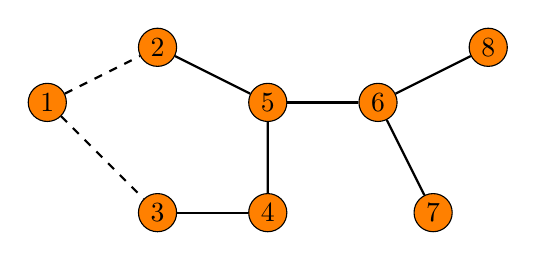
\begin{tikzpicture}[scale = 0.7,
    node/.style={circle, fill=orange, draw, minimum size=1em, inner sep=2pt}]
	    %\draw[gray, very thin] (0,0) grid (6,4);    
	    \node[node] (1) at (0,2) {1};
	    \node[node] (2) at (2,3) {2};
	    \node[node] (3) at (2,0) {3};
	    \node[node] (4) at (4,0) {4};
	    \node[node] (5) at (4,2) {5};
	    \node[node] (6) at (6,2) {6}; 
	    \node[node] (7) at (7,0) {7};
	    \node[node] (8) at (8,3) {8};
	    \draw[thick, -] (2) -- (5);
	    \draw[thick, -] (3) -- (4);
	    \draw[thick, -] (4) -- (5);
	    \draw[thick, -] (5) -- (6);
	    \draw[thick, -] (6) -- (7);
	    \draw[thick, -] (6) -- (8);
	    \draw[thick, dashed] (1) -- (2);
	    \draw[thick, dashed] (1) -- (3);     
    \end{tikzpicture}
    
    {\footnotesize
    \begin{tikzpicture} \draw[thick, -] (0,0.25) -- (0.25,0); \end{tikzpicture} edges of a tree on nodes $\braces{2,\dots, 8}$.
    \begin{tikzpicture} \draw[dashed, -] (0,0.25) -- (0.25,0); \end{tikzpicture} 2 edges from node 1.
    }
    \caption{An example of a 1-tree considering eight nodes} \label{p1c9:fig:1-tree}	
\end{figure}

Once again, it so turns out that several efficient algorithms are known for forming minimal spanning trees, which can be efficiently utilised as a relaxation for the symmetric TSP, that is
%
\begin{align*}
    z_{STSP} = &\mini_{T\subseteq E}\braces{\sum_{e \in T} c_{e} : T \text{ forms a tour}} \geq \\
    z_{1-TREE} = &\mini_{T\subseteq E}\braces{\sum_{e \in T} c_{e} : T \text{ forms a 1-tree}}. 
\end{align*}



\section{Branch-and-bound method}


Relaxations play a major role in solving mixed-integer programming and/or combinatorial optimisation problems. However, they are only part of the framework (specifically, the bounding part of the branch-and-bound method). One still needs to be able to, from the solution of said relaxations, be able to construct a solution to the original problem.

\emph{Branch-and-bound} is an algorithmic strategy that is far broader than mathematical programming and optimisation. In essence, it consists of a \emph{divide-and-conquer} strategy, in which we first break an original problem into smaller and manageable (or solvable) parts and then recombine the solution of these parts into a solution for the original problem.

Specifically, let 
%
\begin{equation*}
	P: z = \maxi_x \braces{c^\top x : x\ \in S}. 
\end{equation*}
%
The working principle behind this strategy is based on the principle formalised in Proposition \ref{p1c9:prop:divide-and-conquer}.

\begin{proposition} \label{p1c9:prop:divide-and-conquer}
    Let $K = \braces{1,\dots,|K|}$ and  $\bigcup_{k \in K} S_k = S$ be a decomposition of $S$. Let $z^k = \maxi_x\braces{c^\top x : x \in  S_k}, \forall k \in K$. Then 
	%
    \begin{equation*}
    	z = \max_{k \in K} \braces{z^k}.	
    \end{equation*}
\end{proposition}

Notice the use of the word \emph{decomposition} in Proposition \ref{p1c9:prop:divide-and-conquer}. Indeed, the principle is philosophically the same, and this connection will be exploited in later chapters when we discuss in more detail the available technology for solving mixed-integer programming problems.

Now, one challenging aspect related with divide-and-conquer approaches is that, in order to be able to find a solution, one might need to repeat several times the strategy based on Proposition \ref{p1c9:prop:divide-and-conquer}, leading to a multi-layered collection of subproblems. To address this issue, such methods typically rely on tree structures called \emph{enumerative trees}, which are simply a representation that allows for keeping track the relationship (represented by branches) between subproblems (represented by nodes).

Figure \ref{p1c9:fig:binary_tree} represents an enumerative tree for a generic problem $S \subseteq \braces{0,1}^3$ in which one must define the value of a three-dimensional binary variable. The subproblems are formed by, at each level, fixing one of the components to zero or one, forming then two subproblems. Any strategy to form subproblems that generate two subproblems (or children) is called a \emph{binary branching}.

\begin{figure}[h]
	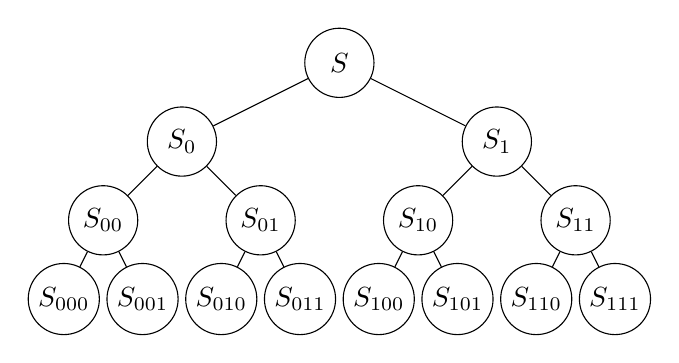
\begin{tikzpicture}[circle, level distance=1cm,
	level 1/.style={sibling distance=4.cm},
	level 2/.style={sibling distance=2.0cm},
	level 3/.style={sibling distance=1.0cm},
	minimum size=2.5em, inner sep=2pt]                
		\node [draw] {$S$}
		child {node [draw] {$S_0$} 
		    child {node [draw] {$S_{00}$}
		        child {node [draw] {$S_{000}$}}
		        child {node [draw] {$S_{001}$}}        
		    }
		    child {node [draw] {$S_{01}$} 
		        child {node [draw] {$S_{010}$}}
		        child {node [draw] {$S_{011}$}}
		    }}
		child { node [draw] {$S_1$} 
		    child {node [draw] {$S_{10}$}
		        child {node [draw] {$S_{100}$}}
		        child {node [draw] {$S_{101}$}}
		    }
		    child {node [draw] {$S_{11}$}
		        child {node [draw] {$S_{110}$}}
		        child {node [draw] {$S_{111}$}}
		    } 
		};    
	\end{tikzpicture}
	\caption{A enumeration tree using binary branching for a problem with three binary variables} \label{p1c9:fig:binary_tree}
\end{figure}
 
Specifically, notice that, at the highest level, we have 
%
\begin{equation*}
	S = S_0\cup S_1 = \braces{x \in S : x_1 = 0} \cup   \braces{x \in S : x_1 = 1}, \\
\end{equation*}
%	
which renders two subproblems. Then, each subproblem is again decomposed each into two children, such that
%
\begin{equation*}	
	S_i = S_{i0} \cup S_{i1} = \braces{x \in S : x_1 = i, x_2 = 0} \cup \braces{x \in S : x_1 = i, x_2 = 1}.\\
\end{equation*}
%	
Finally, once all of the variables are fixed, we arrive at what is called the \emph{leaves} of the tree. These are such that they cannot be further divided, since they immediately yield a candidate solution for the original problem. 
%
\begin{equation*}
	S_{ij} = S_{ij0} \cup S_{ij1} = \braces{x \in S : x_1 = i, x_2 = j, x_3 = 0} \cup \braces{x \in S : x_1 = i, x_2 = j, x_3 = 1}
\end{equation*}
%
Notice that applying Proposition \ref{p1c9:prop:divide-and-conquer}, we can recover an optimal solution to the problem.


\subsection{Bounding in enumerative trees} \label{section_913}

As you may suspect, the strategy of enumerating all possible solutions will quickly become computationally intractable and will most likely not be feasible for mixed-integer programming problems, or any relevant combinatorial optimisation for that matter. That is precisely when the notion of bounding comes to the spotlight: by possessing bound information on our original problem, we might be able to dismiss branches (or prune, in keeping with our tree analogy) from being searched, and hopefully find a solution without the need to exhaustively explore the enumeration tree.

The main principle behind the pruning of branches in enumerative search trees is summarised in Proposition \ref{p1c9:prop:bounding}.	

\begin{proposition} \label{p1c9:prop:bounding}
	Consider the problem $P$ and let $S = \bigcup_{k \in K} S_k$ be a decomposition of $S$ into smaller sets. Let $z^k = \maxi_x\braces{c^\top x : x \in S_k}$ for $k \in K$, and let $\overline{z}^k$ ($\underline{z}^k$) be an upper (lower) bound on $z^k$. Then $\overline{z} = \max_{k \in K} \braces{\overline{z}^k}$ and $\underline{z} = \max_{k \in K} \braces{\underline{z}^k}$.
\end{proposition}

First, notice tat $P$ is a maximisation problem, for which an upper bound is a dual bound, obtained from a relaxation, and a lower bound is a primal bound, obtained from a feasible solution. Proposition \ref{p1c9:prop:bounding} states that the best known primal (lower) bound can be applied \emph{globally} to all of the subproblems $S_k$, $k \in K$. On the other hand, dual (upper) bounds can only be considered valid locally, since only the worst of the upper bounds can be guaranteed to hold globally.

Pruning branches is made possible by combining relaxations and global primal bounds. If, at any moment of the search, the solution of a relaxation of $S_k$ is observed to be \emph{worse} than a known global primal bound, then any further branching from that point onwards would be fruitless, since no solution found from that subproblem could be better than the relaxation for $S_k$. Specifically, we have that
%
\begin{equation*}
	\underline{z} \ge \overline{z}_k \ge \overline{z}_{k'}, \ \forall k' \text{ that is descendent of } k.	
\end{equation*}



\subsection{Linear-programming-based branch-and-bound}

\emph{Branch-and-bound} is the general nomenclature given to methods that operate based on solving relaxations of subproblems and using bounding information to preemptively prune branches in the enumerative search tree. 

The characteristics that define a branch-and-bound method are thus the relaxation being solved (or how bounding is performed), and how subproblems are generated (how branching is performed). In the specific context of (mixed-)integer programming problems, bounding is performed utilising linear programming (LP) relaxations. 

In regards to branching, we employ the following strategy utilising the information from the solution of the LP relaxation. At a given subproblem $S_k$, suppose we have an optimal solution with a fractional component $x^{*k}_j = \overline{x}_j \notin \integers^1$. We can then \emph{branch} $S_k$ into the following subproblems:
	%
    \begin{equation*}
        S_{k1} = S_k \cap \braces{x : x_j \leq \floor{\overline{x_j}}} \text{ and }
        S_{k2} = S_k \cap \braces{x : x_j \geq \ceil{\overline{x_j}}}.
    \end{equation*}
	
Notice that this implies that each of the subproblems will be disjunct (i.e., with no intersection) and have one additional constraint that eliminates the fractional part of the component around the solution of the LP relaxation. 

Bounding can occur in three distinct ways. The first case is when the solution of the LP relaxation happens to be integer and, therefore, optimal for the subproblem itself. In this case, no further exploration along that subproblem is necessary and we say that the node has been \emph{pruned by optimality}.

Figure \ref{p1c9:fig:prune_by_optimality} illustrates the process of pruning by optimality. Each box denotes a subproblem, with the interval denoting known lower (primal) and upper (dual) bounds for the problem and $x$ denoting the solution for the LP relaxation of the subproblem. In Figure \ref{p1c9:fig:prune_by_optimality}, we see a pruning that is caused because a solution to the original (integer) subproblem has been identified by solving its (LP) relaxation, akin to the leaves in the enumerative tree represented in Figure \ref{p1c9:fig:binary_tree}. This can be concluded because the solution of the LP relaxation of subproblem $S_1$ is integer. 

\begin{figure*}[h]
	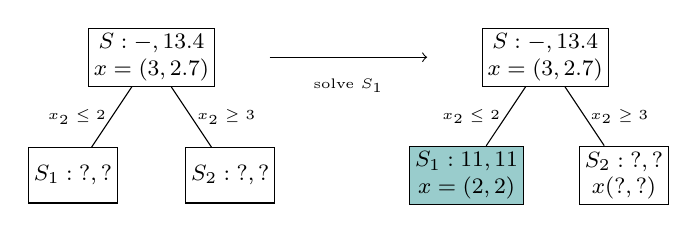
\begin{tikzpicture}[level distance=1.5cm, 
	 level 1/.style={sibling distance=2.0cm}, 
	 level 2/.style={sibling distance=1.5cm}, 
	 minimum size=2em, inner sep=2pt,
	 treenode/.style={draw, align=center, font=\footnotesize}]
	    \node at (0,0) [treenode] {$S:\brackets{-,13.4}$\\$x=(3,2.7)$}
	        child {node [treenode] {$S_1:\brackets{?,?}$}
	        edge from parent node [left, font = \tiny]{$x_2 \leq 2$}
	        }
	        child {node [treenode] {$S_2:\brackets{?,?}$}
	        edge from parent node [right, font = \tiny]{$x_2 \geq 3$}
	        };
	    \draw[->] (1.5,0) -- node[below, font=\tiny]{solve $S_1$} (3.5,0);
	    \node at (5,0) [treenode] {$S:\brackets{-,13.4}$\\$x=(3,2.7)$}
	        child {node [treenode, fill=teal!40] {$S_1:\brackets{11,11}$\\$x=(2,2)$}
	        edge from parent node [left, font = \tiny]{$x_2 \leq 2$}
	        }
	        child {node [treenode] {$S_2:\brackets{?,?}$\\$x(?,?)$}
	        edge from parent node [right, font = \tiny]{$x_2 \geq 3$}};
	 \end{tikzpicture}
	 \caption{An example of pruning by optimality. Since the solution of LP relaxation of subproblem $S_1$ is integer, $x = (2,2)$ must be optimal for $S_1$} \label{p1c9:fig:prune_by_optimality}	
\end{figure*}

Another type of pruning takes place when known global (primal) bounds can be used to prevent further exploration of a branch in the enumeration tree. Continuing the example in Figure \ref{p1c9:fig:prune_by_optimality}, notice that the global lower (primal) bound $\underline{z} = 11$ becomes available and can be transmitted to all subproblems. Now suppose we solve the LP relaxation of $S_2$ and obtain the optimal value of $\overline{z}_2 = 9.7$. Notice that we are precisely in the situation described in Section \ref{section_913}. That is, the nodes descending from $S_2$ (i.e., their descendants) can only yield solutions that have objective function value worse than the dual bound of $S_2$, which, in turn, is worse than a known global primal (lower) bound. Thus, any further exploration among the descendants of $S_2$ would be fruitless in terms of yielding better solutions and can be pruned. This is known as \emph{pruning by bound}, and is illustrated in Figure \ref{p1c9:fig:pruning_by_bound}.

\begin{figure}[h]
	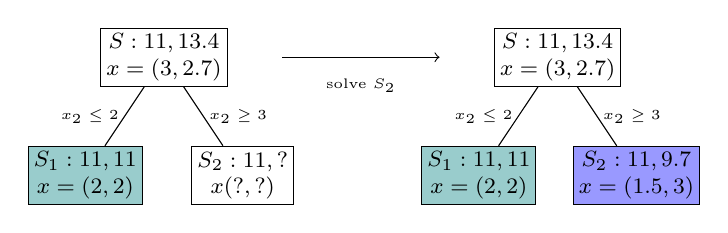
\begin{tikzpicture}[level distance=1.5cm, 
	 level 1/.style={sibling distance=2.0cm}, 
	 level 2/.style={sibling distance=1.5cm}, 
	 minimum size=2em, inner sep=2pt,
	 treenode/.style={draw, align=center, font=\footnotesize}]
	    \node at (0,0) [treenode] {$S:\brackets{11,13.4}$\\$x=(3,2.7)$}
	        child {node [treenode, fill=teal!40] {$S_1:\brackets{11,11}$\\$x=(2,2)$}
	        edge from parent node [left, font = \tiny]{$x_2 \leq 2$}
	        }
	        child {node [treenode] {$S_2:\brackets{11,?}$\\$x(?,?)$}
	        edge from parent node [right, font = \tiny]{$x_2 \geq 3$}};
	    \draw[->] (1.5,0) -- node[below, font=\tiny]{solve $S_2$} (3.5,0);
	    \node at (5,0) [treenode] {$S:\brackets{11,13.4}$\\$x=(3,2.7)$}
	        child {node [treenode, fill=teal!40] {$S_1:\brackets{11,11}$\\$x=(2,2)$}
	        edge from parent node [left, font = \tiny]{$x_2 \leq 2$}
	        }
	        child {node [treenode, fill=blue!40] {$S_2:\brackets{11,9.7}$\\$x=(1.5,3)$}
	        edge from parent node [right, font = \tiny]{$x_2 \geq 3$}};    
	 \end{tikzpicture}
	 \caption{An example of pruning by bound. Notice that the newly found global bound holds for all subproblems. After solving the LP relaxation of $S_2$, we notice that $\overline{z}_2 \le \underline{z}$, which renders the pruning.} \label{p1c9:fig:pruning_by_bound}
\end{figure}

The third type of pruning is called \emph{pruning by infeasibility}, which takes place whenever the branching constraint added to the subproblem renders its relaxation infeasible, implying that the subproblem itself is infeasible (cf. Proposition \ref{p1c9:prop:relaxation_optimality})

Algorithm \ref{p1c9:alg:BB} presents a pseudocode for an LP-based branch-and-bound method. Notice that the algorithm keeps a list $\mathcal{L}$ of subproblems to be solved and requires that a certain rule to select which subproblem is solved next to be employed. This subproblem selection (often referred to as \emph{search strategy}) can have considerable impacts on the performance of the method. Similarly, in case multiple components are found to be fractional, one must be chosen. Defining such \emph{branching priorities} also has consequences to performance. We will discuss these in more depth later on.

Also, recall that we have seen how to efficiently resolve a linear programming problem from an optimal basis once we include an additional constraint (in Chapter \ref{chapter_6}). It so turns out that an efficient dual simplex method is the kingpin of an efficient branch-and-bound method for (mixed)-integer programming problems.

Finally, although we developed the method in the context of integer programming problems, the method can be readily applied to mixed-integer programming problems, with the only difference being that the branch-and-bound steps are only applied to the integer variables while the continuous variables are naturally taken care of in the solution of the LP relaxations.

\begin{algorithm}[h]
	\caption{LP-relaxation-based branch-and-bound} \label{p1c9:alg:BB}
	\begin{algorithmic}[1] %line numbering frequency. 
		\State {\bf initialise.} $\mathcal{L} \gets \braces{S}$, $\underline{z} \gets -\infty$, $\overline{x} \gets -\infty$
		\While {$\mathcal{L} \neq \emptyset$} \label{p1c9:alg:BB_loop}
		    \State select problem $S_i$ from $\mathcal{L}$. $\mathcal{L} \gets \mathcal{L}\setminus\braces{S_i}$. 
		    \State solve LP relaxation of $S_i$ over $P_i$, obtaining $z_{LP}^i$ and $x_{LP}^i$. $\overline{z}^i \gets z_{LP}^i$. 
		    \If {$S_i = \emptyset$} return to step \ref{p1c9:alg:BB_loop}.
		    \ElsIf {$\overline{z}^i \leq \underline{z}$} return to step \ref{p1c9:alg:BB_loop}.    
		    \ElsIf {$x_{LP}^i \in \integers^n$} $\underline{z} \gets \max\braces{\underline{z}, \overline{z}^i}$, $\overline{x} \gets x_{LP}^i$; and return to step \ref{p1c9:alg:BB_loop}
		    \EndIf
		    \State select a fractional component $x_j$ and create subproblems $S_{i1}$ and $S_{i2}$ with formulations $P_{i1}$ and $P_{i2}$, respectively, such that 
		    %
		    \begin{equation*}
		    		P_{i1} = P_i \cup \braces{x_j \leq \floor{\overline{x_j}}} \text{ and } P_{i2} = P_i \cup \braces{x_j \geq \ceil{\overline{x_j}}}.
		    \end{equation*}
		    %
		    \State $\mathcal{L} \gets \mathcal{L} \cup \braces{S_{i1}, S_{i2}}$.
		\EndWhile
		\State {\bf return} ($\overline{x}, \underline{z}$).
	\end{algorithmic}
\end{algorithm}  

Let us finalise presenting a numerical example of the employment of branch-and-bound method to solve an integer programming problem. Consider the problem:
%
\begin{align*}
    \maxi_x z = & 4x_1 - x_2 \\
    \st & 7x_1 - 2x_2 \leq 14 \\
    &x_2 \leq 3 \\
    &2x_1 - 2x_2 \leq 3 \\
    &x \in \integers^2_+
\end{align*} 
%
We start by solving its LP relaxation, as represented in Figure \ref{p1c9:fig:example_LP_relaxation_solution}. We obtain the solution $x_{LP}=(20/7, 3)$ with objective value of $z=59/7$. As the first component of $x$ is fractional, we can generate subproblems by branching the node into subproblems $S_1$ and $S_2$, where
%
\begin{align*}
	& S_1 = S \cap \braces{x : x_1 \leq 2} \\
	& S_2 = S \cap \braces{x : x_1 \geq 3}.
\end{align*}
%
The current enumerative (or branch-and-bound) tree representation is depicted in Figure \ref{p1c9:fig:example_bb_tree_1}.

\begin{figure}[h]
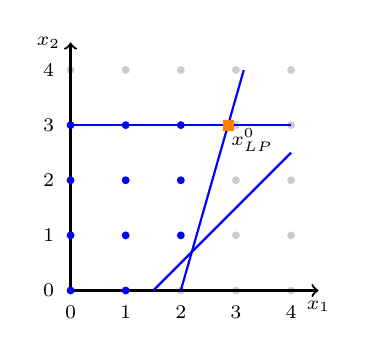
\begin{tikzpicture}[scale = 0.7,
	point/.style={circle, fill=gray!40, inner sep=1pt},
	feas point/.style={circle, fill=blue, inner sep=1pt}]
	\foreach \x in {0,...,4}{
		\foreach \y in {0,...,4} {
			\node[point] (\x,\y) at (\x, \y) {};
	}}
	\foreach \x in {0,...,4}{
		\node[font=\scriptsize] at (\x,-0.4) {$\x$};
	}
	\foreach \y in {0,...,4}{
		\node[font=\scriptsize] at (-0.4,\y) {$\y$};
	}                      
	\draw[thick, <->] (4.5,0) node[below, font=\scriptsize]{$x_1$} -- (0,0) -- (0,4.5) node[left, font=\scriptsize]{$x_2$};    
	\draw[domain=3/2:4, thick,variable=\x,blue] plot ({\x},{-3/2 + \x});
	\draw[domain=2:22/7, thick,variable=\x,blue] plot ({\x},{-7 + 3.5*\x});
	\draw[domain=0:4, thick,variable=\x,blue] plot ({\x},{3});
	\node[fill=orange, inner sep=2pt] (LP) at (20/7, 3) {};          
	\node[font=\scriptsize, below right,inner sep=1pt] at (LP) {$x_{LP}^0$};
	\node[feas point] at (0,0){};
	\node[feas point] at (1,0){};
	\foreach \x in {0,...,2}{ 
	\foreach \y in {1,...,3}{        
	\node[feas point] at (\x,\y){};
	}}
	\end{tikzpicture}
	\caption{LP relaxation of the problem $S$}\label{p1c9:fig:example_LP_relaxation_solution}	
\end{figure}


\begin{figure}[h]
	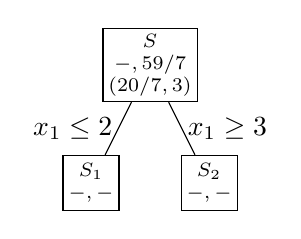
\begin{tikzpicture}[level distance=1.5cm, 
	 level 1/.style={sibling distance=1.5cm}, 
	 level 2/.style={sibling distance=1.5cm}, 
	 minimum size=2em, inner sep=2pt,
	 treenode/.style={draw, align=center, font=\scriptsize}]
	    \node at (0,0) [treenode] {$S$\\$\brackets{-,59/7}$\\$(20/7,3)$}
	        child {node [treenode] {$S_1$\\$\brackets{-,-}$}
	        edge from parent node [left]{$x_1 \leq 2$}
	            }
	        child {node [treenode] {$S_2$\\$\brackets{-,-}$}
	        edge from parent node [right]{$x_1 \geq 3$}
	        };
	 \end{tikzpicture}
	\caption{The branch-and-bound tree after branching $S$ onto $S_1$ and $S_2$} \label{p1c9:fig:example_bb_tree_1}	
\end{figure}

Suppose we arbitrarily choose to solve the relaxation of $S_1$ next. Notice that this subproblem consists of the problem $S$, with the added constraint $x_1 \le 2$. The feasible region and solution of the LP relaxation of $S_2$ is depicted in Figure \ref{p1c9:fig:example_LP_relaxation_solution_2}. Since we again obtain a new fractional solution $x_{LP}^1 = (2,1/2)$, we must branch on the second component, forming the subproblems 
%
\begin{align*}
    & S_{11} = S_1 \cap \braces{x : x_2 = 0} \\
    & S_{12} = S_1 \cap \braces{x : x_2 \geq 1}.
\end{align*}

\begin{figure}[h]
	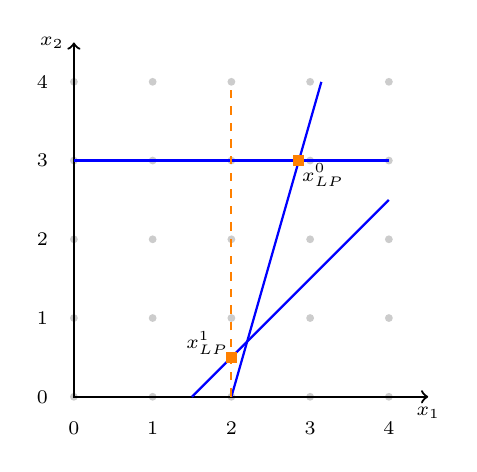
\begin{tikzpicture}[scale = 1,
		point/.style={circle, fill=gray!40, inner sep=1pt},
		feas point/.style={circle, fill=blue, inner sep=1pt}]
		\foreach \x in {0,...,4}{
		  \foreach \y in {0,...,4} {
		      \node[point] (\x,\y) at (\x, \y) {};
		  }}
		\foreach \x in {0,...,4}{
		  \node[font=\scriptsize] at (\x,-0.4) {$\x$};
		}
		\foreach \y in {0,...,4}{
		  \node[font=\scriptsize] at (-0.4,\y) {$\y$};
		}                      
		\draw[thick, <->] (4.5,0) node[below, font=\scriptsize]{$x_1$} -- (0,0) -- (0,4.5) node[left, font=\scriptsize]{$x_2$};    
		\draw[domain=3/2:4, thick,variable=\x,blue] plot ({\x},{-3/2 + \x});
		\draw[domain=2:22/7, thick,variable=\x,blue] plot ({\x},{-7 + 3.5*\x});
		\draw[domain=0:4, thick,variable=\x,blue] plot ({\x},{3});
		\draw[domain=0:4, thick,orange, dashed] (2,0) -- (2,4);
		\node[fill=orange, inner sep=2pt] (LP) at (20/7, 3) {};          
		\node[font=\scriptsize, below right,inner sep=1pt] at (LP) {$x_{LP}^0$};
		\node[fill=orange, inner sep=2pt] (LP2) at (2, 1/2) {};          
		\node[font=\scriptsize, above left,inner sep=1pt] at (LP2) {$x_{LP}^1$};
	\end{tikzpicture}
	\caption{LP relaxation of subproblem $S_1$} \label{p1c9:fig:example_LP_relaxation_solution_2}		
\end{figure}

Notice that, at this point, our list of active subproblems is formed by $\mathcal{L} = \braces{S_1, S_{11}, S_{12}}$. Our current branch-and-bound tree is represented in Figure \ref{p1c9:fig:example_bb_tree_2}. 

Suppose we arbitrarily choose to first solve $S_2$. Once can see that this would render an infeasible subproblem, since the constraint $x_2 \ge 3$ does not intersect with the original feasible region and, thus, $S_2$ can be pruned by infeasibility.

\begin{figure}[h]
	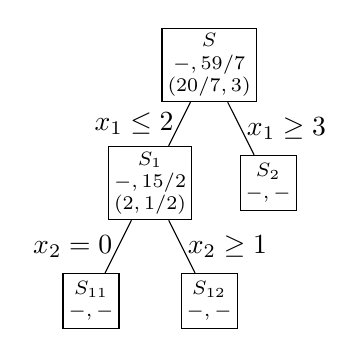
\begin{tikzpicture}[level distance=1.5cm, 
     level 1/.style={sibling distance=1.5cm}, 
     level 2/.style={sibling distance=1.5cm}, 
     minimum size=2em, inner sep=2pt,
     treenode/.style={draw, align=center, font=\scriptsize}]
        \node at (0,0) [treenode] {$S$\\$\brackets{-,59/7}$\\$(20/7,3)$}
            child {node [treenode] {$S_1$\\$\brackets{-,15/2}$\\$(2,1/2)$}
                child {node [treenode] {$S_{11}$\\$\brackets{-,-}$}
                edge from parent node [left]{$x_2 = 0$}
                }
                child {node [treenode] {$S_{12}$\\$\brackets{-,-}$}
                edge from parent node [right]{$x_2 \geq 1$}
                }
            edge from parent node [left]{$x_1 \leq 2$}
                }
            child {node [treenode] {$S_2$\\$\brackets{-,-}$}
            edge from parent node [right]{$x_1 \geq 3$}
            };
     \end{tikzpicture}
     \caption{The branch-and-bound tree after branching $S_1$ onto $S_{11}$ and $S_{12}$} \label{p1c9:fig:example_bb_tree_2}
\end{figure}

Next, we choose to solve the LP relaxation of $S_{12}$, which yields an integer solution $x_{LP}^{12} = (2,1)$. Therefore, an optimal solution for $S_{12}$ was found, meaning that a global primal (lower) bound has been found and can be transmitted to the whole branch-and-bound tree. Solving $S_{11}$ next, we obtain the solution $x_{LP}^{11} = (3/2, 0)$ with optimal value $z = 6$. Since a better global primal (lower) bound is known, we can prune $S_{11}$ by bound. As there are no further nodes to be explored, the solution for the original problem is the best (and, in this case, the single) integer solution found in the process (cf. Proposition \ref{p1c9:prop:divide-and-conquer}), $x^* = (2,1)$, $z^* = 7$. Figure \ref{p1c9:fig:example_LP_relaxation_solution_3} illustrates the feasible region of the subproblems and their respective optimal solutions, while Figure \ref{p1c9:fig:example_bb_tree_3} presents the final branch-and-bound tree with all branches pruned.

\begin{figure}[h]
	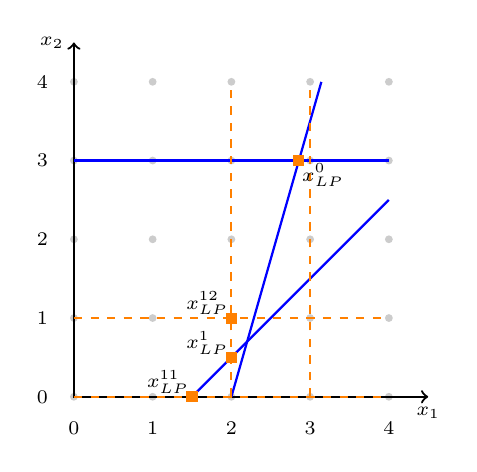
\begin{tikzpicture}[scale = 1,
	point/.style={circle, fill=gray!40, inner sep=1pt},
	feas point/.style={circle, fill=blue, inner sep=1pt}]
	\foreach \x in {0,...,4}{
	  \foreach \y in {0,...,4} {
	      \node[point] (\x,\y) at (\x, \y) {};
	  }}
	\foreach \x in {0,...,4}{
	  \node[font=\scriptsize] at (\x,-0.4) {$\x$};
	}
	\foreach \y in {0,...,4}{
	  \node[font=\scriptsize] at (-0.4,\y) {$\y$};
	}                      
	\draw[thick, <->] (4.5,0) node[below, font=\scriptsize]{$x_1$} -- (0,0) -- (0,4.5) node[left, font=\scriptsize]{$x_2$};    
	\draw[domain=3/2:4, thick, variable=\x, blue] plot ({\x},{-3/2 + \x});
	\draw[domain=2:22/7, thick, variable=\x, blue] plot ({\x},{-7 + 3.5*\x});
	\draw[domain=0:4, thick, variable=\x, blue] plot ({\x},{3});
	\draw[domain=0:4, thick, variable=\x, orange, dashed] plot ({\x},{0});
	\draw[domain=0:4, thick, variable=\x, orange, dashed] plot ({\x},{1});
	\draw[thick, orange, dashed] (2,0) -- (2,4);
	\draw[thick, orange, dashed] (3,0) -- (3,4);
	\node[fill=orange, inner sep=2pt] (LP) at (20/7, 3) {};          
	\node[font=\scriptsize, below right,inner sep=1pt] at (LP) {$x_{LP}^0$};
	\node[fill=orange, inner sep=2pt] (LP2) at (2, 1/2) {};          
	\node[font=\scriptsize, above left,inner sep=1pt] at (LP2) {$x_{LP}^1$};
	\node[fill=orange, inner sep=2pt] (LP3) at (2, 1) {};          
	\node[font=\scriptsize, above left,inner sep=1pt] at (LP3) {$x_{LP}^{12}$};
	\node[fill=orange, inner sep=2pt] (LP4) at (3/2, 0) {};          
	\node[font=\scriptsize, above left,inner sep=1pt] at (LP4) {$x_{LP}^{11}$};
	\end{tikzpicture}
	\caption{LP relaxations of all subproblems. Notice that $S_{11}$ and $S_{12}$ includes the constraints $x_1 \le 2$ from the parent node $S_1$}	\label{p1c9:fig:example_LP_relaxation_solution_3}
\end{figure}

\begin{figure}[h]
	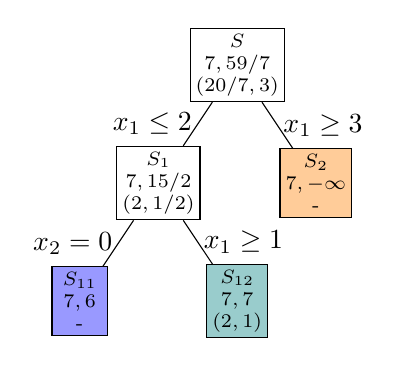
\begin{tikzpicture}[level distance=1.5cm, 
     level 1/.style={sibling distance=2cm}, 
     level 2/.style={sibling distance=2cm}, 
     minimum size=2em, inner sep=2pt,
     treenode/.style={draw, align=center, font=\scriptsize}]
        \node at (0,0) [treenode] {$S$\\$\brackets{7,59/7}$\\$(20/7,3)$}
            child {node [treenode] {$S_1$\\$\brackets{7,15/2}$\\$(2,1/2)$}
                child {node [treenode, fill=blue!40] {$S_{11}$\\$\brackets{7,6}$\\-}
                edge from parent node [left]{$x_2 = 0$}
                }
                child {node [treenode, fill=teal!40] {$S_{12}$\\$\brackets{7,7}$\\$(2,1)$}
                edge from parent node [right]{$x_1 \geq 1$}
                }
            edge from parent node [left]{$x_1 \leq 2$}
                }
            child {node [treenode, fill = orange!40] {$S_2$\\$\brackets{7,-\infty}$\\-}
            edge from parent node [right]{$x_1 \geq 3$}
            };
     \end{tikzpicture}
     \caption{The final branch-and-bound tree} \label{p1c9:fig:example_bb_tree_3}
\end{figure}

Notice that in this example, the order in which we solved the subproblems was crucial for pruning by bound the subproblem $S_{11}$, only possible because we happened to solve the LP relaxation of $S_{12}$ first and that happened to yield a feasible solution and associated primal bound. This illustrates an important aspect associated with the branch and bound method: having good feasible solutions available early on in the process increases the likelihood of performing more pruning by bound, which is highly desirable in terms of computational savings (and thus, performance). We will discuss in more detail the impacts of different search strategies later on when we consider this and other aspects involved in the implementation of mixed-integer programming solvers.

\pagebreak 

\section{Exercises}

\subsection*{Problem 9.1: Uncapacitated Facility Location (UFL)}
\textbf{(a)}  Let $N = \{1,\dots,n\}$ be a set of potential facilities and $M = \{1,\dots,m\}$ a set of clients. Let $y_j = 1$ if facility $j$ is opened, and $y_j = 0$ otherwise. Moreover, let $x_{ij}$ be the fraction of client $i$'s demand satisfied from facility $j$. The UFL can be formulated as the mixed-integer problem (MIP): 

\begin{align}
 \text{(UFL-W)} : \quad &\mini_{x,y} \sum_{j\in N} f_jy_j + \sum_{i\in M}\sum_{j\in N} c_{ij}x_{ij} \label{IP:1}\\
       &\st\nonumber \\
       &\quad \sum_{j\in N}x_{ij} = 1, &\forall i \in M,\label{IP:2}\\
       &\quad \sum_{i\in M}x_{ij} \leq my_j, &\forall  j \in N,\label{IP:3}\\
       &\quad x_{ij} \geq 0, &\forall i \in M, \forall j \in N,\label{IP:4}\\
       &\quad y_j \in \{0,1\}, &\forall j\in N,\label{IP:5}
\end{align}

where $f_j$ is the cost of opening facility $j$, and $c_{ij}$ is the cost of satisfying client $i$'s demand from facility $j$. Consider an instance of the UFL with opening costs $f=(4,3,4,4,7)$ and client costs

\begin{equation*}
 (c_{ij}) = \left(
	\begin{array}{ccccc}
		12 & 13 & 6 & 0  & 1 \\
		8  & 4  & 9 & 1  & 2 \\
		2  & 6  & 6 & 0  & 1 \\
		3  & 5  & 2 & 1  & 8 \\
		8  & 0  & 5 & 10 & 8 \\
		2  & 0  & 3 & 4  & 1
	\end{array}
 \right)
\end{equation*}

Implement (the model) and solve the problem with Julia using JuMP.

\textbf{(b)} An alternative formulation of the UFL is of the form

\begin{align}
 \text{(UFL-S)} : \quad &\mini_{x,y} \sum_{j\in N}f_jy_j + \sum_{i\in M}\sum_{j\in N}c_{ij}x_{ij}\label{SIP:1}\\
       &\st\nonumber \\
       &\quad \sum_{j\in N}x_{ij} = 1, &\forall i \in M,\label{SIP:2}\\
       &\quad x_{ij} \leq y_j, &\forall  i\in M, \forall j \in N,\label{SIP:3}\\
       &\quad x_{ij} \geq 0, &\forall i \in M, \forall j \in N,\label{SIP:4}\\
       &\quad y_j \in \{0,1\}, &\forall j\in N.\label{SIP:5}
\end{align}


Linear programming (LP) relaxations of these problems can be obtained by relaxing the binary constraints $y_j\in \{0,1\}$ to $0 \leq y_j \leq 1$ for all $j \in N$. For the same instance as in part (a), solve the LP relaxations of UFL-W and UFL-S and compare the optimal costs of the LP relaxations against the optimal integer cost obtained in part (a).

\pagebreak
\subsection*{Problem 9.2: LP-based branch-and-bound method}
Consider the following IP problem and its standard form

\begin{minipage}[c]{0.4\textwidth}
\begin{align*}
\text{(IP)} \quad z = \text{max} \quad & 4x_1 - x_2      \\
                   \st \quad & 7x_1 -  2x_2    \leq 14\\
                             & x_2 \leq 3 \\
		       		         & 2x_1 -     2x_2 \leq 3 \\
		     	             & x_1,x_2 \in \integers_+
\end{align*}
\end{minipage}
\begin{minipage}{0.5\textwidth}
\begin{table}[H]
	\centering
	\begin{tabular}{V{0.3cm} V{0.6cm} V{0.2cm} r V{0.1cm} V{0.1cm} V{0.4cm} V{0.2cm} r r}
        $\text{(IP)}$  & z =   &     max & \multicolumn{3}{c}{$4x_1 - x_2$}                \vspace{5pt}               \\
		               & $\st$ &  7$x_1$ &  $+$\ 2$x_2$ & $+ \ x_3$ &           &           & $=$ &  14 &             \\
					   &       &         &        $x_2$ &           & $+ \ x_4$ &           & $=$ &   3 &             \\
					   &       &  2$x_1$ &  $-$\ 2$x_2$ &           &           & $+ \ x_5$ & $=$ &   3 & \vspace{5pt}\\ 
	                   & \multicolumn{8}{c}{$x_1, \dots, x_5 \in \integers_+$}   
	\end{tabular}
\end{table}
\end{minipage}\\

Solve the IP problem by LP-based branch and bound, i.e., use LP relaxations to compute dual (upper) bounds. Use Dual Simplex to efficiently solve the subproblem of each node starting from the optimal basis of the previous node. Recall that the LP relaxation of IP is obtained by relaxing the variables $x_1,\dots,x_5\in \integers_+$ to $x_1,\dots,x_5 \geq 0$.

\emph{Hint:} The initial dual bound $\overline{z}$ is obtained by solving the LP relaxation of IP at the root node $S$. Let $[\underline{z},\overline{z}]$ be the lower and upper bounds of each node. The optimal tableau and the initial Branch \& Bound  tree with only the root node $S$ is shown below. 

\vspace{5pt}

\renewcommand{\arraystretch}{1.2}
\setlength{\tabcolsep}{8pt}

\begin{minipage}{0.72\textwidth}
\begin{tabular}{r|c|ccccc}
       & -$z$  & $x_1$ & $x_2$ & $x_3$ & $x_4$ & $x_5$\\
     \hline
       & -59/7 & 0     & 0     & -4/7  & -1/7  & 0\\
     \hline
$x_1=$ & 20/7 & 1     & 0     &  1/7  & 2/7   & 0\\
$x_2=$ &  3   & 0     & 1     &  0    &  1    & 0\\
$x_5=$ & 23/7 & 0     & 0     & -2/7  & 10/7  & 1 
\end{tabular}
\end{minipage}
\begin{minipage}{0.23\textwidth}
\footnotesize
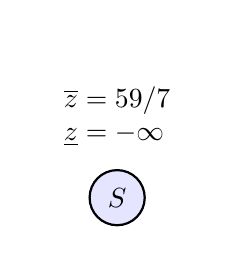
\begin{tikzpicture}[thick, label distance=-1.5mm, level 1/.style={sibling distance=20mm},
					level 2/.style={sibling distance=20mm},  level distance=12mm]

    \tikzstyle{every node}=[draw,circle,minimum size=7mm]

    \node[opacity=1,
    	  fill=blue!10,
    	  label={[label distance=-14pt]above:\begin{tabular}{l} 
    										 $\overline{z}  = 59/7$\\
    										 $\underline{z} = -\infty$
    									     \end{tabular}}](root){$S$};
\end{tikzpicture}
\end{minipage}\\[5pt]

You can proceed by branching on the fractional variable $x_1$ and imposing either $x_1\leq 2$ or $x\geq 3$. This creates two new subproblems $S_1 = S\cap \{x_1\leq 2\}$ and $S_2 = S\cap \{x_1\geq 3\}$ in the Branch \& Bound tree that can be solved efficiently by Dual Simplex starting from the optimal tableau of $S$ shown above, by first adding the new constraint $x_1\leq 2$ for $S_1$ or $x_1\geq 3$ for $S_2$ to the optimal tableau. The Dual Simplex can be applied immediately if the new constraint is always written in terms of non-basic variables before adding it to the tableau as a new row, possibly multiplying the constraint by $-1$ if needed. 


\subsection*{Problem 9.3: Employing the branch-and-bound method graphically}
Consider the following integer programming problem $IP$:

%\begin{table}[H]
%	\centering
%	\begin{tabular}{V{0.4cm} r V{0.1cm} r V{0.1cm} l}
%		$\text{(IP)}$  & \multicolumn{4}{l}{z = max \ $x_1\ +\ 2x_2$}  \vspace{10pt}\\ 
%		        $\st$  & $-\ 3x_1$ & $+$ & 4$x_2$ & $\leq$ &  4                     \\
%		               &    3$x_1$ & $+$ & 2$x_2$ & $\leq$ & 11                     \\
%		               &    2$x_1$ & $-$ &  $x_2$ & $\leq$ &  5        \vspace{10pt}\\
%		               & \multicolumn{2}{l}{$x_1, x_2 \in \integers_+$}   
%	\end{tabular}
%\end{table}

\begin{align*}
	(IP) : \maxi z =~& x_1 + 2x_2   \\
	\st & -3x_1 + 4x_2 \le 4 \\
		& 3x_1 + 2x_2 \le 11 \\
		& 2x_1 - x_2 \le 5   \\
		& x_1, x_2 \in \integers_+
\end{align*}

Plot (or draw) the feasible region of the linear programming (LP) relaxation of the problem $IP$, then solve the problems using the figure. Recall that the LP relaxation of $IP$ is obtained by replacing the integrality constraints $x_1,x_2\in \integers_+$ by linear nonnegativity $x_1,x_2\geq 0$ and upper bounds corresponding to the upper bounds of the integer variables ($x_1,x_2\leq 1$ for binary variables). 

\begin{itemize}
	\item[(a)] What is the optimal cost $z_{LP}$ of the LP relaxation of the problem $IP$? What is the optimal cost $z$ of the problem $IP$?
	\item[(b)] Draw the border of the convex hull of the feasible solutions of the problem $IP$. Recall that the convex hull represents the \emph{ideal} formulation for the problem $IP$.
	\item[(c)] Solve the problem $IP$ by LP-relaxation based branch-and-bound. You can solve the LP relaxations at each node of the branch-and-bound tree graphically. Start the branch-and-bound procedure without any primal bound.
\end{itemize}






